\chapter{Kết quả nghiên cứu}
%Mô tả ngắn gọn các kết quả nghiên cứu, thực nghiệm. Bàn luận về điểm mạnh, điểm yếu của mô hình được xây dựng trong luận văn. So sánh kết quả thu được trong quá trình nghiên cứu, thực nghiệm của đề tài và đối chiếu với kết quả nghiên cứu, thực nghiệm của các tác giả khác một cách khách quan. Nêu lên điểm nổi bật, khác biệt của luận văn đối với các nghiên cứu khác.

\section{Các tập dữ liệu được sử dụng}
\subsection{Tập dữ liệu LRW \cite{lrw}}

Tập dữ liệu LRW là tập dữ liệu được xây dựng bởi một nhóm nghiên cứu từ trường Đại học Oxford và sở hữu bởi hãng tin tức BBC. Đây là tập dữ liệu lớn, với những đoạn video ngắn được cắt từ những đoạn video được phát trên kênh BBC và được thu trong môi trường tự nhiên. Tập dữ liệu LRW có hơn 1 triệu video khác nhau, mỗi video có độ dài 1.16 giây, gồm 29 khung hình. Những video này được chia làm 1000 từ vựng, mỗi từ vựng được nói bởi hơn 1000 người khác nhau. Tổng cộng, tập dữ liệu LRW chứa gần 1000 giờ video. Tuy nhiên, do được thu trong môi trường tự nhiên, tín hiệu trong video có độ nhiễu nhất định. Âm thanh trong video có thể nghe rõ lời nói, tuy nhiên một số lượng không nhỏ video bị lẫn tiếng ồn và các tạp âm khác. Về mặt hình ảnh, video có hình ảnh rõ nét, lấy điểm trên đầu mũi của người đang nói làm trung tâm, vì vậy, với các video mà người nói có sự cử động ở đầu như xoay hay lắc đầu, video sẽ bị rung lắc mạnh để giữ điểm đầu mũi ở giữa khung hình. Mặt người trong video được quay ở nhiều vị trí khác nhau và có thể lệch về một phía (quay từ phía bên trái, bên phải, hoặc lệch theo chiều dọc gương mặt). Với mỗi từ ngữ, tập dữ liệu đã chia sẵn thành 3 tập tập huấn luyện, tập kiểm chứng và tập kiểm thử với số lượng video tương ứng cho mỗi loại là 1000-50-50.

\begin{figure}[H]
    \centering
    \includegraphics[width=12cm]{./content/materials/lrw.png}
    \caption{Ảnh trích xuất từ các video trong tập dữ liệu LRW}
\end{figure}

\subsection{Tập dữ liệu GRID \cite{grid}}

Tập dữ liệu GRID là tập dữ liệu được tạo ra từ phòng nghiên cứu của Đại học Sheffield tại Anh. Tập dữ liệu này được tạo ra để hỗ trợ cho việc phân tích và nghiên cứu gương mặt người khi nói, bao gồm các nghiên cứu về nhận thức gương mặt thông qua giọng nói và nhận diện giọng nói. Tập dữ liệu chứa 1000 câu, được nói bởi 34 người khác nhau. Như vậy, tập dữ liệu này chứa 34000 video với chất lượng cao, mỗi video có độ dài 3 giây. Những câu được nói rất đơn giản, với cú pháp: <động từ (4 từ)> <màu sắc (4 từ)> <giới từ (4 từ)> <chữ cái (25 chữ)> <số (10 số)> <trạng từ (4 từ)>. Các cụm từ giống hệt nhau về mặt cú pháp đã nêu ở trên (ví dụ như câu "place green at B 4 now"), được phát âm rõ và đọc với tốc độ bình thường, âm thanh được thu ở môi trường kín, không nhiễu. Hình ảnh trong video rõ nét, được quay với phông nền xanh với điều kiện ánh sáng tốt. Mặt người khi nói ít chuyển động (ít xoay, ít lắc đầu) và được quay trực diện. Gương mặt người khi nói không biểu lộ cảm xúc và người nói chớp mắt một cách tự nhiên. Các video trong tập GRID được chia thành 3 tập huấn luyện, tập kiểm chứng và tập kiểm thử với tỉ lệ 90\%-5\%-5\% tương ứng.

Do tập dữ liệu LRW có độ nhiễu cao, nên ta sẽ sử dụng tập dữ liệu GRID để tính cột mốc gương mặt chuẩn $l_{standard}$ như đã miêu tả ở phân \ref{sec:preprocess_audio_lm}. Cột mốc gương mặt chuẩn $l_{standard}$ tuy được tính toán trên tập GRID nhưng sẽ được sử dụng để chuẩn hóa cột mốc gương mặt cho cả tập GRID và tập LRW. Cách thức chuẩn hóa cột mốc khuôn mặt trong luận văn lấy ý tưởng từ bài báo \cite{gen_face_landmark} và được chỉnh sửa để phù hợp với việc xử lý dữ liệu cho bài toán.

\begin{figure}[H]
    \centering
    \includegraphics[width=12cm]{./content/materials/grid.png}
    \caption{Ảnh trích xuất từ các video trong tập dữ liệu GRID}
\end{figure}

\section{Các độ đo được sử dụng để đánh giá kết quả tạo sinh hình ảnh}\label{sec:metrics}

Việc tạo sinh dữ liệu hình ảnh mặt người dựa theo giọng nói hiện tại vẫn chưa có một độ đo nào làm chuẩn mực để đánh giá chất lượng tạo sinh hình ảnh, thậm chí một số nghiên cứu về vấn đề này trên các tạp chí uy tín cũng được xuất bản mà không có độ đo chuẩn để đánh giá mô hình một cách cụ thể \cite{chung} \cite{wav2pix}.

Một video mặt người đang nói trong tự nhiên có thể có các chuyển động đầu, mắt, và biểu cảm gương mặt tùy ý. Tuy nhiên video được tạo sinh có thể có thể tạo ra chuyển động đầu theo một hướng khác, chớp mắt ở thời điểm khác và biểu cảm gương mặt theo một cách khác. Vì vậy một độ đo lý tưởng là một độ đo không bị ảnh hưởng bởi các chuyển động của đầu, chớp mắt và biểu cảm gương mặt mà nên tập trung vào nội dung và bản chất của hình ảnh. Việc sử dụng hàm mất mát L2 trong việc tạo sinh ảnh có thể làm cho hình ảnh ổn định và đẹp hơn, tuy nhiên khó có thể dùng hàm mất mát L2 để đánh giá hình ảnh tạo sinh một cách công bằng do hàm mất mát L2 sẽ gây ra giá trị mất mát lớn nếu chuyển động của đầu trong video được tạo sinh không giống với video gốc. Ta có thể dùng độ đo PSNR (Peak Signal-to-Noise) để tính toán độ sai lệch cho từng điểm ảnh dựa vào hàm mất mát L2. Tuy nhiên, như đã giải thích ở trên, độ đo này bỏ qua tính tự nhiên trong quá trình chuyển động của đầu và gương mặt trong ảnh tạo sinh mà chỉ chú trọng vào sự giống nhau ở từng điểm ảnh trên video gốc vào video tạo sinh. Vì vậy đây không phải là một độ đo thật sự tốt để đánh giá chất lượng tạo sinh hình ảnh.

Một độ đo tốt hơn PSNR cho việc tính toán sự tương đồng giữa video gốc và video tạo sinh là SSIM (structural similarity index measure) \cite{ssim}. Độ đo này được sử dụng để đo sự tương đồng về mặt cấu trúc giữa hai hình ảnh, nhằm giảm bớt sự cứng nhắc của các phép so sánh chính xác \cite{psrn_ssim}. Độ đo này được tính toán bằng cách so sánh các điểm ảnh xung quanh của một điểm ảnh trên ảnh gốc và ảnh được tạo sinh với ba kênh gồm kênh tương phản, kênh độ chói và kênh cấu trúc. Ý tưởng về mặt so sánh cấu trúc giữa hai hình ảnh được đưa ra từ việc một điểm ảnh sẽ luôn có sự liên kết chặt chẽ với các điểm ảnh xung quanh nó. Sự liên kết này hàm chứa thông tin quan trọng về cấu trúc của những vật thể trong ảnh. Bên cạnh đó, độ đo này cũng lưu ý đến sự chói sáng và sự khác biệt về độ tương phản của ảnh trong những vùng có sự thay đổi. Hình sau là một ví dụ so sánh giữa sai số L2 và SSIM:

\begin{figure}[H]
    \centering
    \includegraphics[width=15cm]{./content/materials/l2_ssim.png}
    \caption{So sánh giữa sai số L2 và SSIM}
\end{figure}

Để đo lường độ sắc nét của hình ảnh được tạo sinh, ta sử dụng độ đo CPBD (Cumulative 
Probability of Blur Detection) \cite{cpbd}. Bằng cách kết hợp ý tưởng của việc phát hiện vùng mờ bằng xác suất tích lũy với định nghĩa về vùng mờ vừa được chú ý (just noticeable blur) thành một mô hình tổng hợp xác suất, CPBD đánh giá độ sắc nét của hình ảnh trên quan điểm tri giác, phù hợp với nhận thức của con người.

Trong luận văn này, ta sử dụng SSIM để đo lường chất lượng hình ảnh của video được tạo sinh và CPBD để đo lường độ sắc nét cho các khung hình

\section{Quá trình thực hiện}

Chi tiết các môi trường huấn luyện và chạy các thí nghiệm được liệt kê ở bảng \ref{table:hardware}

\begin{table}[h]
    \centering
    \begin{tabular}{c | c | c}
    \hline 
    &\textbf{Máy A} & \textbf{Máy B}\\
    \hline
    \textbf{CPU} & Intel Xeon & Intel Core I5 8600K\\
    \textbf{Bộ nhớ} & 24GB & 32GB\\
    \textbf{GPU} & NVIDIA TESLA V100 & NVIDIA Geforce RTX 3070\\
    \textbf{Ổ cứng} & 160GB SSD & 768GB NVME SSD + 2TB HDD\\
    \textbf{OS} & N/A(Colab Pro) & Ubuntu 20.04\\
    \textbf{Ngôn ngữ} & Python 3.7 & Python 3.7\\
    \textbf{Framework} & Pytorch 1.8 & Pytorch 1.8\\
    \hline
    \end{tabular}
    \caption{Các môi trường được sử dụng trong việc tiền xử lý dữ liệu, huấn luyện và thực hiện thí nghiệm}
    \label{table:hardware}
\end{table}

Máy A được sử dụng trong việc huấn luyện hệ thống mạng GANs bao gồm mạng tạo sinh hình ảnh và mạng phân biệt. Trong khi máy B được sử dụng để làm những công đoạn còn lại bao gồm tiền xử lý dữ liệu, huấn luyện mạng tạo sinh cột mốc gương mặt và tiến hành chạy các thí nghiệm, đo đạc thông số. Các số liệu sau đây đều được ghi nhận trên các thiết bị này. 

Việc huấn luyện mạng như đã nói được chia làm hai bước. Bước đầu tiên là huấn luyện mạng tạo sinh cột mốc gương mặt và bước thứ hai là huấn luyện hệ thống mạng GANs. Các thông số và kết quả huấn luyện mạng tạo sinh cột mốc gương mặt trên máy B cho hai tập dữ liệu được thể hiện qua bảng sau:

\begin{table}[h]
    \centering
    \begin{tabular}{c | c | c}
    \hline 
    &\textbf{GRID} & \textbf{LRW}\\
    \hline
    \textbf{Bộ tối ưu} & Adam & Adam\\
    \textbf{Kích thước bó} & 100 & 100\\
    \textbf{Hệ số học} & 0.001 & 0.0002\\
    \textbf{Thời gian huấn luyện} & 5 phút & 70 phút\\
    \textbf{$\mathcal{L}_{landmark}$} & $4.9200 \times 10^{-4}$ & $2.012 \times 10^{-4}$\\
    \hline
    \end{tabular}
    \caption{Chi tiết huấn luyện mạng tạo sinh cột mốc gương mặt. Giá trị mất mát (trên tập kiểm thử) và thời gian huấn luyện được ghi nhận tại vòng lặp cho ra mô hình tối ưu}
    \label{table:landmark_decoder_training_detail}
\end{table}

Mạng tạo sinh cột mốc gương mặt có cấu trúc đơn giản và huấn luyện nhanh. Do tập dữ liệu LRW có kích thước rất lớn và cấu trúc dữ liệu phức tạp hơn nên ta cái đặt hệ số học nhỏ hơn. Đồng thời thời gian huấn luyện mạng này cùng lâu hơn mạng GRID nhiều lần. Tuy nhiên mạng này cho ra giá trị mất mát MSE nhỏ hơn do có nhiều dữ liệu để học hơn. Bước thứ hai trong việc huấn luyện mạng là huấn luyện hệ thống mạng GANs. Việc huấn luyện này được tiến hành trên máy A. Chi tiết về việc huấn luyện mạng được liệt kê trong bảng sau:

\begin{table}[h]
    \centering
    \begin{tabular}{c | c | c}
    \hline 
    &\textbf{GRID} & \textbf{LRW}\\
    \hline
    \textbf{Bộ tối ưu} & Adam & Adam\\
    \textbf{Kích thước bó} & 12 & 17\\
    \textbf{Hệ số học} & 0.0002 & 0.0002\\
    \textbf{Thời gian huấn luyện} & 5 giờ 20 phút & 250 giờ\\
    \textbf{$\mathcal{L}_{pix}$} & $4.1575 \times 10^{-2}$ & $6.8502 \times 10^{-2}$\\
    \textbf{$\mathcal{L}_{gans-dis}$} & $0.9964$ & $0.6931$\\
    \textbf{$\mathcal{L}_{gans-landmark}$} & $7.6990 \times 10^{-2}$ & $5.2412 \times 10^{-2}$\\
    \textbf{$\mathcal{L}$} & $1.4892$ & $1.4306$\\
    \hline
    \end{tabular}
    \caption{Chi tiết huấn luyện mạng GANs. Giá trị mất mát (trên tập kiểm thử) và thời gian huấn luyện được ghi nhận tại vòng lặp cho ra mô hình tối ưu}
    \label{table:gans_training_detail}
\end{table}

Theo như bảng trên, việc huấn luyện mạng GANs cho tập dữ liệu LRW có thời gian rất lâu, mạng này được huấn luyện đến vòng lặp thứ 25 (mỗi vòng lặp khoảng 10 giờ) thì hội tụ. Tuy nhiên tác giả đã huấn luyện thêm đến vòng lặp thứ 40 để chắc chắn không rơi vào vùng tối ưu cục bộ. Các giá trị hàm mất mát cho thấy giá trị mất mát tổng ở cả hai tập GRID và LRW ($\mathcal{L}$) là gần bằng nhau. Tuy nhiên, trong các giá trị mất mát thành phần thì giá trị $\mathcal{L}_{gans-landmark}$ và $\mathcal{L}_{gans-dis}$ ở tập LRW có giá trị thấp hơn do tập LRW có nhiều dữ liệu hơn để học, nên mạng phân biệt của tập LRW có khả năng phân biệt thật giả và sinh ra cột mốc gương mặt tốt hơn hẳn so với tập GRID. Ngược lại, ở tập GRID, giá trị $\mathcal{L}_{pix}$ của tập này thấp hơn so với tập LRW do tính chất dữ liệu của nó. Đối với tập GRID, như đã nói, các video trong tập này được quay trong phòng thí nghiệm và được canh chỉnh sao cho gương mặt không xoay và không di chuyển. Vì vậy mạng dễ học để tạo sinh chính xác hình ảnh hơn để có hàm mất mát L1 thấp hơn hẳn tập LRW.


\section{Các kết quả trên tập dữ liệu GRID}

Đầu tiên, ta thử tạo sinh cột mốc gương mặt từ giọng nói sử dụng mạng tạo sinh cột mốc gương mặt vừa được huấn luyện ở các bước trên. Kết quả tạo sinh cột mốc gương mặt được thể hiện ở hình dưới.

\begin{figure}[H]
    \centering
    \includegraphics[width=15cm]{./content/materials/grid_examples-landmark.png}
    \caption{Kết quả tạo sinh cột mốc gương mặt trên tập GRID, cột mốc màu đỏ là cột mốc được tạo sinh, màu xanh là cột mốc được trích xuất từ hình ảnh gốc}
\end{figure}

So sánh cột mốc gương mặt được tạo sinh (cột mốc màu đỏ) và cột mốc gốc (màu xanh) ta thấy mạng đã dự đoán tương đối tốt chuyển động của cột mốc gương mặt theo lời nói dựa vào độ trùng lắp của các cột mốc. Ta đưa các cột mốc vừa được tính toán vào mạng tạo sinh kèm với hình ảnh mẫu và cột mốc gương mặt của ảnh mẫu, ta sẽ tạo ra được chuỗi hình ảnh mặt người đang nói. Mạng phân biệt sẽ không được sử dụng trong quá trình sinh ảnh này. Sau đây là một số ví dụ tạo sinh ảnh trên tập GRID

\begin{figure}[H]
    \centering
    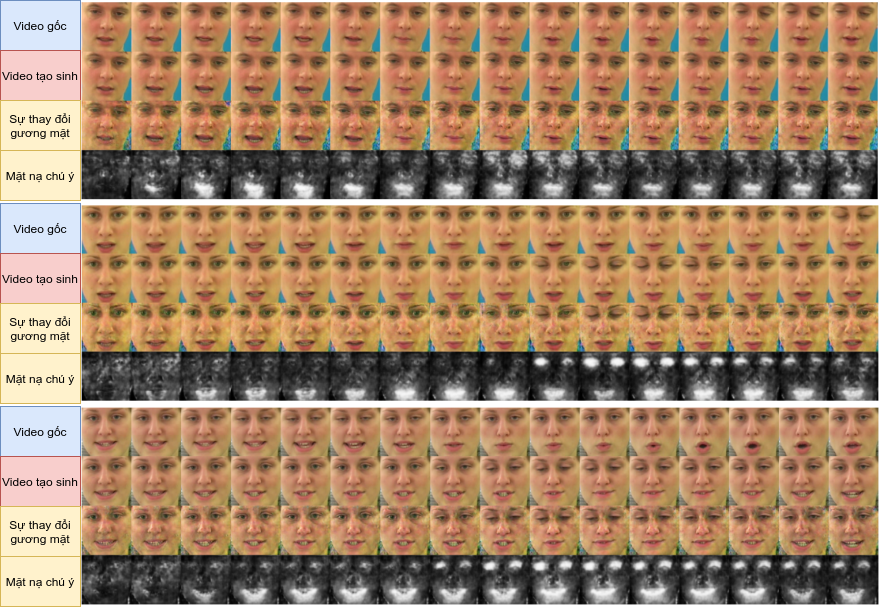
\includegraphics[width=15cm]{./content/materials/grid_examples-face.png}
    \caption{Kết quả tạo sinh gương mặt theo giọng nói trên tập GRID}
\end{figure}

Theo kết quả tạo sinh ta thấy, hình ảnh tạo sinh có khẩu hình miệng phù hợp với tiếng nói và gần giống với video gốc. Mặt nạ chú ý chủ yếu tập trung vào vùng mắt và miệng, trong khi các phần khác trên gương mặt và phông nền dường như không được chú ý đến. Một số video ngoài khả năng cử động miệng, có thể sinh ra hành động chớp mắt và hành động này diễn ra một cách ngẫu nhiên. Hành động chớp mắt diễn ra trong vòng 6 đến 7 khung hình, tương ứng với khoảng thời gian 240ms đến 280ms, phù hợp với hành động chớp mắt trong thực tế của con người. Trên video mô tả sự thay đổi gương mặt $p'_{image}$, chỉ có các vùng được chú ý đến mới được tạo sinh hình ảnh rõ ràng, các vùng còn lại thường sinh ra nhiễu. Điều này rất hợp lý vì trên thực tế, các vùng không được chú ý đến sẽ không đóng góp nhiều vào giá trị mất mát của mạng, nên những vùng này cũng không cần được tạo sinh một cách hoàn chỉnh.

Tác giả cũng đã chạy thử để tạo sinh hình ảnh gương mặt người đang nói trong điều kiện ảnh thực tế. Hình ảnh sau là ảnh người mẫu được thử nghiệm và kết quả tạo sinh thực tế cho đoạn âm thanh với câu nói: "set red by z5 soon".
\begin{figure}[H]
    \centering
    \includegraphics[width=5cm]{./content/materials/khang.png}
    \caption{Ảnh người mẫu trong thử nghiệm chạy thực tế}
\end{figure}

\begin{figure}[H]
    \centering
    \includegraphics[width=16cm]{./content/materials/khang_gen.png}
    \caption{Video được tạo sinh bởi mô hình GRID}
\end{figure}

Ta thấy mặc dù bị gây nhiễu bởi khẩu trang và kính, nhưng mô hình vẫn tạo sinh được video có chất lượng tương đối tốt và vẫn giữ nguyên được đặc trưng gương mặt người nói. Phần được chú ý chủ yếu vẫn là phần miệng, chuyển động của miệng tương đồng với từ ngữ được nói trong đoạn âm thanh.

\section{Các kết quả trên tập dữ liệu LRW}
Tiến hành các bước tạo sinh tương tự như trên tập dữ liệu GRID, ta thu được các kết quả tạo sinh cột mốc gương mặt tốt hơn so với tập GRID. Điều này đã được giải thích ở phần trên, do tập LRW là tập dữ liệu rất lớn, nên mạng có nhiều dữ liệu hơn để học về âm thanh và cột mốc gương mặt.

\begin{figure}[H]
    \centering
    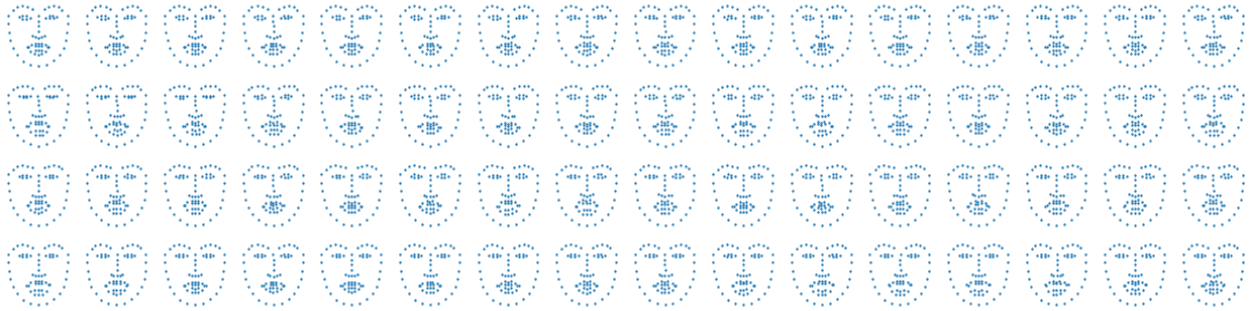
\includegraphics[width=15cm]{./content/materials/lrw_examples-landmark.png}
    \caption{Kết quả tạo sinh cột mốc gương mặt trên tập LRW, cột mốc màu đỏ là cột mốc được tạo sinh, màu xanh là cột mốc được trích xuất từ hình ảnh gốc}
\end{figure}

Hình sau thể hiện kết quả tạo sinh video khi cho mô hình tạo sinh ảnh trên tập kiểm thử với 3 trường hợp: ảnh mẫu được chuẩn hóa tốt, ảnh đầu vào bị lệch, và ảnh đầu vào được quay một bên mặt.

\begin{figure}[H]
    \centering
    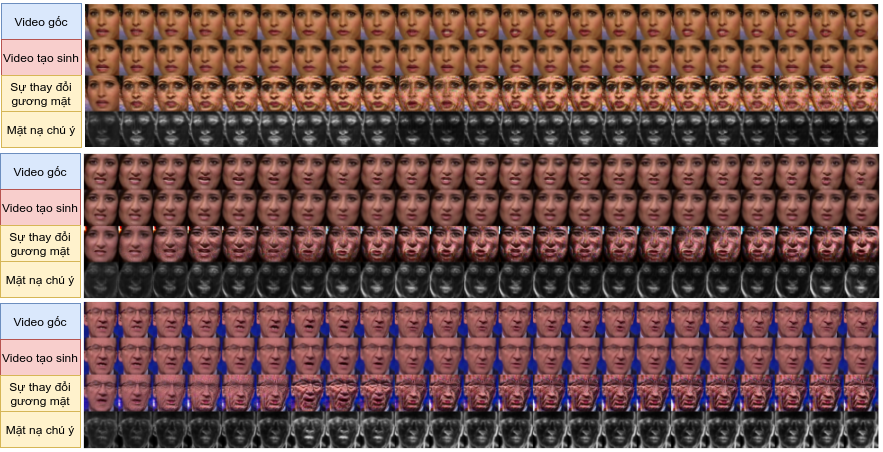
\includegraphics[width=15cm]{./content/materials/lrw_examples-frontal.png}
    \caption{Kết quả tạo sinh gương mặt theo giọng nói trên tập LRW, trường hợp ảnh đầu vào là hình ảnh chiếu thẳng mặt người nói, mặt người được canh bốn góc, mũi nằm ở giữa khung hình}
\end{figure}

\begin{figure}[H]
    \centering
    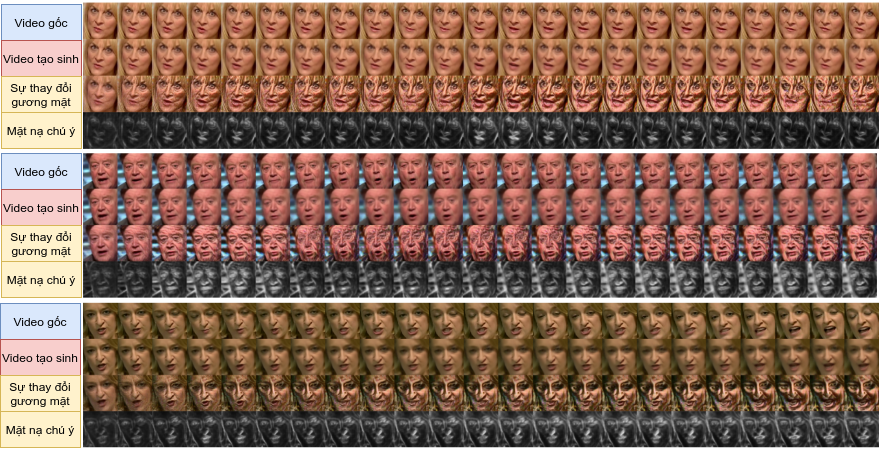
\includegraphics[width=15cm]{./content/materials/lrw_examples-miss_aligned.png}
    \caption{Kết quả tạo sinh gương mặt theo giọng nói trên tập LRW, trường hợp ảnh đầu vào là hình ảnh bị lệch, mặt người nằm ở 1 phía trên khung hình}
\end{figure}

\begin{figure}[H]
    \centering
    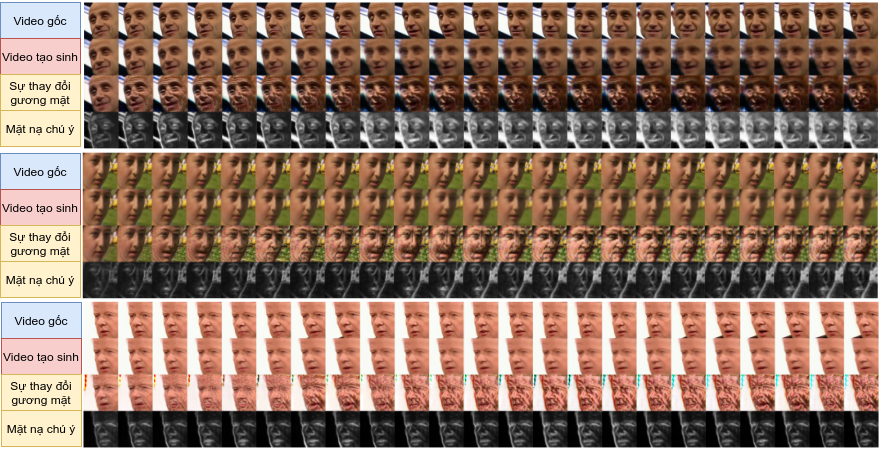
\includegraphics[width=15cm]{./content/materials/lrw_examples-half_face.png}
    \caption{Kết quả tạo sinh gương mặt theo giọng nói trên tập LRW, trường hợp ảnh đầu vào là hình ảnh lệch hẳn về một bên mặt}
\end{figure}

Hình ảnh trên cho thấy, giống như trong tập dữ liệu GRID, phần mắt và miệng trên gương mặt là phần được chú ý nhiều nhất. Các phần khác của khuôn mặt trong hình  $p'_{image}$ cũng không được tạo sinh một cách hoàn chỉnh. Tuy nhiên, do tập dữ liệu LRW có góc quay rất đa dạng nên khi tạo sinh hình ảnh ở nhiều góc độ khác nhau của gương mặt, ta thấy mạng cho kết quả tốt nhất khi tạo sinh ảnh mặt người mẫu được chụp theo hướng chính diện, mặt người được chuẩn hóa tốt và lấp đầy khung hình. Cũng do sự đa dạng của góc quay trên tập LRW, mạng đã không học được cách chớp mắt như trong mô hình của tập GRID.

Tác giả cũng đã thử tạo sinh video với hình ảnh thực tế trên mô hình này và mang lại kết quả khả quan. Hình ảnh người mẫu và video tạo sinh cho câu nói "set white to g2 please" được thể hiện ở hai hình sau:

\begin{figure}[H]
    \centering
    \includegraphics[width=5cm]{./content/materials/eny.png}
    \caption{Ảnh người mẫu trong thử nghiệm chạy thực tế}
\end{figure}

\begin{figure}[H]
    \centering
    \includegraphics[width=16cm]{./content/materials/eny_gen.png}
    \caption{Video được tạo sinh bởi mô hình LRW}
\end{figure}

Qua thử nghiệm trên ta thấy, mô hình đã tạo sinh tương đối tốt hình ảnh người mẫu đang phát âm các từ ngữ trong câu. Khẩu hình miệng được tạo sinh khớp với âm thanh, mặt người mẫu không bị biến dạng và vẫn giữ được đặc trưng khuôn mặt theo thời gian. Khi thử nghiệm hình ảnh của gương mặt này trên mô hình của tập GRID, video được tạo sinh  có chất lượng không tốt, hình ảnh tạo sinh có chuyển động nhưng những chuyển động này không hợp lý. Điều này có thể giải thích là do khối lượng dữ liệu trên mô hình GRID quá ít, nên mạng chưa có đủ thông tin để tổng quát hóa bài toán cho mọi đầu vào.

\section{So sánh mô hình với các nghiên cứu khác}\label{sec:comparision}

Như đã trình bày ở phần \ref{sec:metrics}, ta sẽ sử dụng độ đo SSIM và CPBD để đánh giá và so sánh mô hình trong nghiên cứu này với các mô hình khác trên hai tập dữ liệu GRID và LRW. Bảng \ref{table:metrics_result} cho thấy phép đo đạc và so sánh giữa các mô hình tạo sinh hình ảnh bằng âm thanh.

\begin{table}[h]
    \centering
    \begin{tabular}{c | c | c | c | c}
    \hline 
    \multirow{2}{*}{\textbf{Phương pháp}} & \multicolumn{2}{c|}{\textbf{GRID}} & \multicolumn{2}{c}{\textbf{LRW}}\\
    \cline{2-5}
    & SSIM & CPBD & SSIM & CPBD\\
    \hline
    \textbf{Zakharov et al \cite{zakharov}} & 0.54 & 0.19 & 0.42 & 0.11 \\
    \textbf{Chung et al \cite{chung}} & 0.41 & \textbf{0.22} & 0.34 & \textbf{0.21} \\
    \textbf{Baseline (Chen et al) \cite{chen2019}} & 0.41 & 0.08 & 0.38 & 0.07 \\
    \hline
    \hline
    \textbf{Ours} & \textbf{0.72} & 0.12 & \textbf{0.54} & 0.06 \\
    \hline
    \end{tabular}
    \caption{So sánh với các mạng có cùng mục tiêu về độ đo SSIM và CPBD. Dữ liệu trong bảng được lấy từ bài khảo sát \cite{chen_survey}}
    \label{table:metrics_result}
\end{table}

Qua bảng \ref{table:metrics_result} ta thấy, việc áp dụng và chỉnh sửa phương pháp chuẩn hóa cột mốc gương mặt từ nghiên cứu \cite{gen_face_landmark} vào mô hình của nghiên cứu \cite{chen2019} đã mang lại hiệu quả tốt. Việc chuẩn hóa đầu vào khi tạo sinh cột mốc gương mặt giúp làm tăng độ đo SSIM lên đáng kể, điều này có nghĩa là so với phương pháp cũ, video được tạo sinh giờ đây có cấu trúc tương đồng hơn với video gốc về mặt cảm quan. Chuyển động của mắt, miệng và cả gương mặt trong video tạo sinh có độ ăn khớp với video gốc cao hơn đáng kể so với các nghiên cứu khác. Nhận diện gương mặt người nói trong video tạo sinh cũng được giữ nguyên và không bị biến dạng, các đặc điểm và chi tiết trên gương mặt vẫn được giữ nguyên so với hình ảnh người mẫu ban đầu.

Do việc tạo sinh một cột mốc gương mặt chuẩn và chính xác là tiền đề rất quan trọng trong việc tạo sinh hình ảnh. Cột mốc gương mặt cũng quyết định phần nhiều khẩu hình miệng khi nói, nên việc chuẩn hóa tốt hơn cột mốc gương mặt ở mạng sinh cột mốc là yếu tố then chốt, ảnh hưởng trực tiếp đến kết quả tạo sinh hình ảnh. Nghiên cứu \cite{chen2019} có sử dụng phương pháp chuẩn hóa, nhưng phương pháp này vẫn còn đơn giản và chủ yếu dựa vào phép biến đổi PCA để loại bỏ các chuyển động không mong muốn trên gương mặt (như lắc, xoay đầu làm cho mắt, mũi miệng bị dịch chuyển mạnh). Trong khi đó, với phương pháp được đề xuất trong luận văn, những chuyển động không mong muốn trên được loại bỏ ngay tại bước tiền xử lý qua các phép biến đổi được nêu ở phần \ref{sec:preprocess_audio_lm}. Điều này giúp cho hệ thống mạng GANs ở phía sau có được thông tin chuẩn xác hơn, dễ học hơn để làm cơ sở cho việc tạo sinh gương mặt người nói.

Tuy nhiên, việc chuẩn hóa video đầu vào có thể được thực hiện chưa được tốt trên tập LRW. Trên thực tế, một số video sau khi được chuẩn hóa trên tập LRW có hiện tượng bị nhảy hình, làm đứt gãy tính thời gian của video và làm cho nó trở nên không được mượt mà. Điều này kết hợp với việc sử dụng hàm mất mát L1 cho bộ tạo sinh hình ảnh làm cho video được tạo sinh trên mô hình của tập LRW không có độ nét tốt (CPBD = 0.06), nhất là những video có góc quay gương mặt lệch hẳn về một bên. Đối với tập dữ liệu GRID có tính ổn định về mặt chuyển động của khung hình, CPBD tăng đáng kể.
